\chapter{Simulazioni numeriche e metodologie per l'analisi dati}

\section{Setup simulativo} \label{sec:Setup_sim}
L'obiettivo di questa tesi è studiare l'evoluzione dei dischi circum-stellari al variare dei parametri della binaria. Per questo motivo le simulazioni effettuate prendono in considerazione solamente un disco alla volta, mentre il secondo corpo è posto oltre i confini della regione simulata.

Le coordinate utilizzate per le simulazioni sono quelle cilindriche, con sistema di riferimento fisso (ossia dotato di velocità angolare $\Omega_R\,=\,0$) centrato sulla stella attorno alla quale orbita il disco. Lavoriamo con un sistema di unità scale-free: la massa del corpo centrale $M_\ast$ e la costante di gravitazione universale $G$ assumono sempre valori pari ad uno.
\'E necessario utilizzare una risoluzione spaziale elevata in modo tale che le equazioni differenziali caratteristiche del problema in analisi vengano risolte con elevata precisione: il numero di divisioni radiali $n_r$ che abbiamo utilizzato sono 384, mentre quelle angolari $n_\varphi$ 1152. Entrambe le partizioni sono lineari.

L'estensione della griglia in unità di semiasse maggiore della binaria $a$ varia a seconda dell'oggetto che stiamo prendendo in considerazione: vogliamo lasciare che il disco abbia spazio per espandersi e raggiungere le proprie dimensioni caratteristiche, ma vorremmo evitare che gran parte del dominio simulato risulti vuoto in quanto FARGO3D fa fatica a gestire regioni con densità molto basse ($\sigma\sim\,10^{-40}$).
Per questo motivo è necessario modificare il raggio massimo (a volte anche quello minimo) della griglia per ogni simulazione: per determinare i valori di $r_{min}$ ed $r_{max}$ abbiamo effettuato delle run di 20 orbite a bassa risoluzione. Le dimensioni delle griglie utilizzate sono riportate in Appendice~\ref{appendiceC}. 
Per tutte le simulazioni effettuate abbiamo lavorato con aspect-ratio costante $h/r\,=\,0.05$, valore coerente con le osservazioni (vedi Sezione \ref{sec:mod_disc}).

\subsection{Condizione iniziale}

Il sistema deve essere inizializzato a $t\,=\,0$. Dato che FARGO3D non è in grado di gestire regioni spaziali vuote, è necessario che la densità sia diversa da zero in tutta la griglia.
Per tempi successivi all'istante iniziale, il sistema attraversa una fase di transitorio durante la quale la condizione a $t\,=\,0$ viene modificata per giungere, dopo alcune orbite della binaria, ad una configurazione quasi stabile.
Siamo interessati a determinare quale sia la condizione iniziale computazionalmente ottimale che consenta di ridurre al minimo i tempi d'esecuzione.

Una possibile scelta per il profilo di densità $\sigma(r,\,t=0)$ potrebbe essere quella di avere densità costante in tutta la regione simulata. Dato che alcune zone della griglia devono svuotarsi, lavorare con una tale condizione iniziale comporterebbe la formazione di spirali ed onde di densità intense: tali perturbazioni sono delicate da gestire e richiedono tempi di esecuzione più lunghi a causa dei limiti stringenti imposti dalla \textit{Courant condition} (vedi Sottosezione \ref{subsec:cond_CFL}).

Un modo per evitare tali problematiche consiste nello specializzare il profilo di densità facendo sì che ci sia più materiale a raggi piccoli: tale regione sarà quella che poi ospiterà il disco. 
Una possibile scelta per $\sigma(r,\,t=0)$ è:
\begin{equation}
\sigma(r,\,0)\,=\,\begin{cases}
\sigma_0 \qquad \qquad\,\,\,\,r\,<\,r_0\\
\sigma_0\cdot10^{-5} \qquad r\,\geq\,r_0\\
\end{cases}
\label{eq:condin_dens_gr}
\end{equation}
dove $\sigma_0$ è una densità costante pari a $10^{-4}.$  In Figura \ref{fig:cond_in_sim_gr} è riportato l'andamento di $\sigma(r,\,0)$: notiamo la presenza di un netto gradino per $r\,=\,r_0$.
\begin{figure}[h]
    \centering
    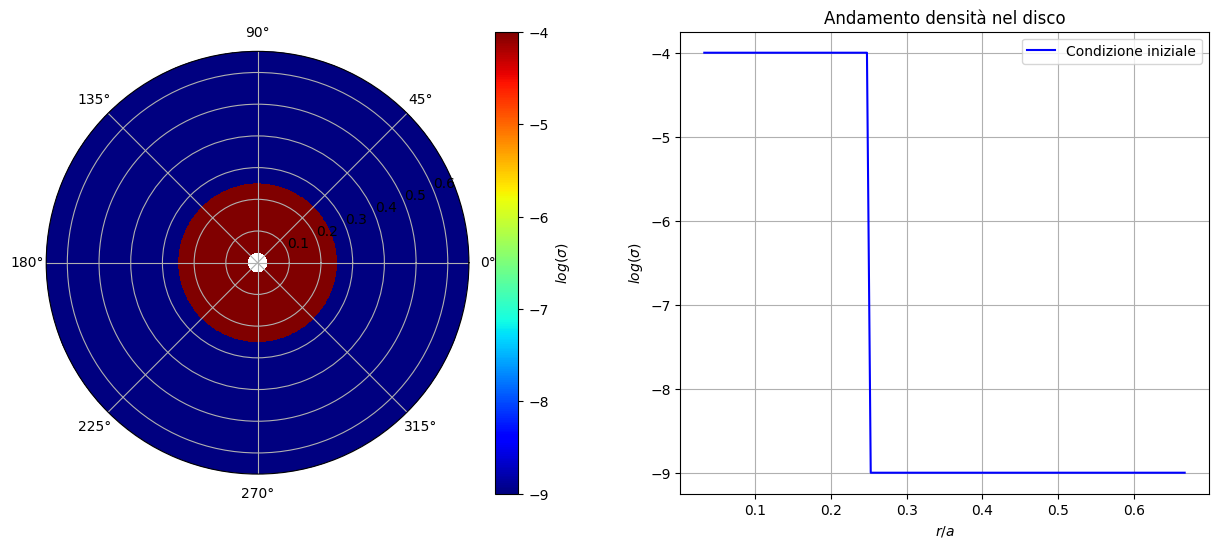
\includegraphics[width=\textwidth]{Immagini/Simulazioni/CondizioneIniziale_grad.png}
    \caption{Esempio di condizione iniziale del sistema: si nota un netto gradino per $r\,=\,r_0$.}
    \label{fig:cond_in_sim_gr}
\end{figure}
Una seconda scelta possibile consiste in un profilo di densità continuo che non presenti gradienti infiniti come il caso precedente.
Fissato un certo valore di raggio $r_0$, la densità iniziale $\sigma(r,\,0)$ è data da:
\begin{equation}
\sigma(r,\,0)\,=\,\begin{cases}
\sigma_0 \cdot (1\,+\,10^{-5}) \qquad \qquad \qquad \qquad \qquad r\,<\,r_0 \\
\sigma_0 \cdot \left\{\exp{[-(r\,-\,r_0)^3]}\,+\,10^{-5}\right\} \qquad \quad r\,\geq\, r_0
\end{cases}
\label{eq:condin_dens}
\end{equation}
\'In \eqref{eq:condin_dens} è necessaria la presenza del termine $10^{-5}$ per far si che il profilo di densità non sia eccessivamente troncato all'outer edge della griglia. In Figura \ref{fig:cond_in_sim} è riportato un esempio di condizione iniziale con profilo continuo e derivabile.

\begin{figure}[h]
    \centering
    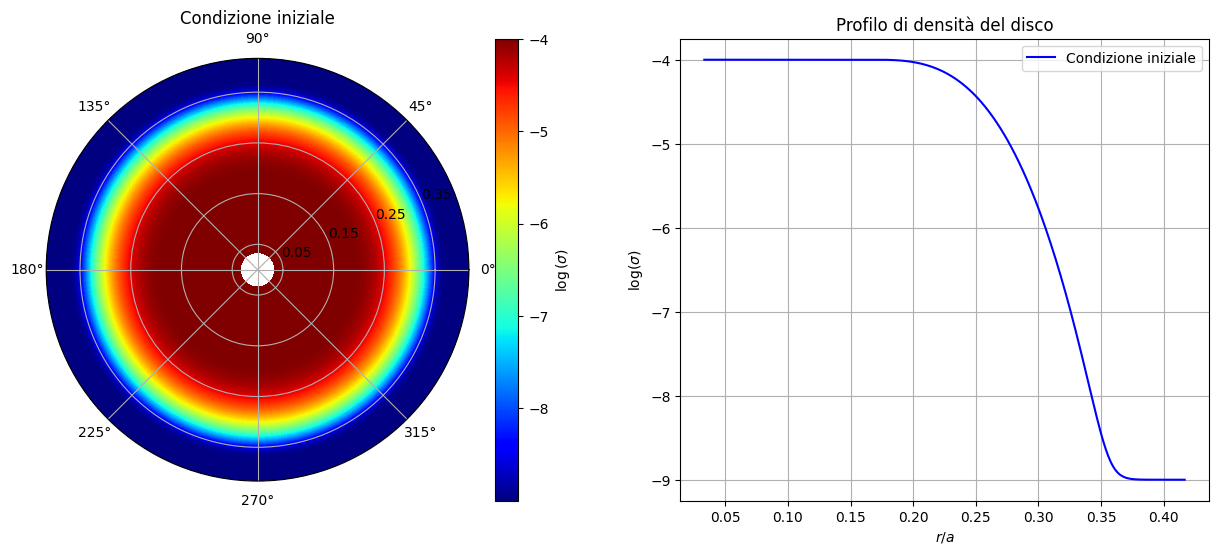
\includegraphics[width=\textwidth]{Immagini/Simulazioni/CondizioneIniziale.png}
    \caption{Esempio di condizione iniziale del sistema: si nota il profilo di densità continuo caratterizzato dall'assenza di gradienti infiniti.}
    \label{fig:cond_in_sim}
\end{figure}
Abbiamo effettuato dei test per determinare quale fosse la scelta migliore fra le due opzioni precedentemente esposte: abbiamo osservato che situazioni caratterizzate dalla presenza di gradienti infiniti (o comunque molto elevati) come la condizione iniziale a gradino generavano più artefatti transienti con un aumento dei tempi d'esecuzione.
Di conseguenza abbiamo optato per la $\sigma(r,\,0)$ dettata dalla \eqref{eq:condin_dens}, che è stata utilizzata per tutte le simulazioni presenti in questa tesi.


\subsection{Condizioni al contorno}

La griglia presenta due frontiere:
\begin{list}{\textbf{-}}{\setlength{\itemsep}{0cm}}
    \item interna, per $r\,=\,r_{min}$;
    \item esterna, per $r\,=\,r_{max}$
\end{list}
\'E necessario lavorare con delle condizioni al contorno che siano tali da non influenzare il fenomeno in analisi e che abbiano una giustificazione di natura fisica: cruciale è la scelta della boundary condition per $v_r$. \\

\textbf{Frontiera interna}\\

\'E fondamentale scegliere correttamente la condizione all'inner boundary perché non deve interferire con il troncamento. Ricordiamo che $r_{min}$ non deve essere scelto troppo piccolo per evitare che le condizioni sul singolo time-step evolutivo siano troppo stringenti, rendendo inefficiente dal punto di vista computazionale la simulazione (vedi Sottosezione \ref{subsec:Fargo_al}).

Alla frontiera interna abbiamo utilizzato una BC \textit{open} per la velocità radiale: tale scelta è migliore rispetto ad una 'inner boundary' antisimmetrica poiché non comporta la riflessione di materiale al bordo griglia ed evita la produzione di onde di densità artificiali, che possono risultare problematiche per lo studio del troncamento.
L'utilizzo di una condizione \textit{open} ad $r_{min}$ comporta la formazione di una cavità artificiale all'interno del disco (vedi Figura \ref{fig:cav_int}).
Il materiale che si muove secondo orbite ellittiche viene tolto dalla regione simulata a periastro determinando la presenza di una regione svuotata ad apoastro.
Questo svuotamento della porzione di griglia adiacente alla frontiera interna non costituisce una problematica per le simulazioni che vogliamo effettuare. La cavità artificiale non influenza le proprietà globali del disco, cosa che succederebbe con le onde di densità che si creerebbero nel caso di BC antisimmetrica.
\begin{figure}[h]
    \centering
    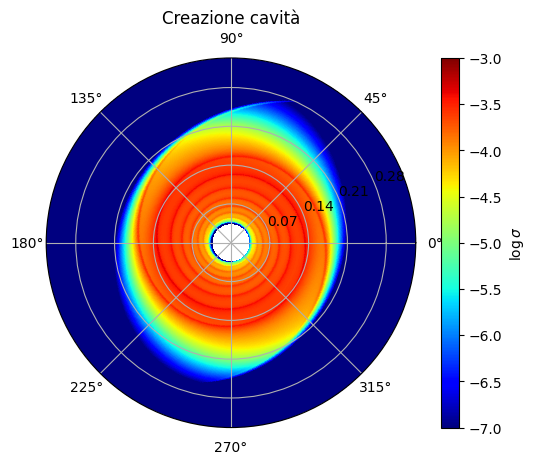
\includegraphics[width=0.55\textwidth]{Immagini/Simulazioni/FormazioneCavita.png}
    \caption{Utilizzo della condizione interna open. La regione adiacente ad $r_{min}$ è di colorazione blu, che corrisponde a valori di densità bassi.}
    \label{fig:cav_int}
\end{figure}
La condizione utilizzata per la densità è \textit{Keplerian2Ddens}, mentre per la velocità azimutale è \textit{Keplerian2Dvazim}.\\

\textbf{Frontiera esterna} \\

Come nel caso della frontiera interna, anche nel caso di quella esterna è necessario imporre una 'boundary condition' per $v_r$ che non influenzi l'evoluzione dinamica del sistema: abbiamo lavorato con una condizione \textit{open} anche ad $r_{max}$.

Per poter procedere in questo senso abbiamo dovuto implementare una nuova BC che abbiamo nominato \textit{OPENOUTER}.\\

OPENOUTER:

\hspace{2cm} Staggered: $|(a>0.0?\,a:\,0.0)|(a>0.0?\,a:\,0.0)|a|$\\

dove la velocità radiale viene posta a zero nelle ghost-cell se negativa nella cella reale: ciò accade perché $v_r$ , per essere uscente dalla griglia ad $r_{max}$, deve essere positiva. La condizione che abbiamo implementato dovrebbe lavorare analogamente a quella \textit{open} ad $r_{min}$, ossia consentire l'uscita di materiale dalla regione simulata, ma non permetterne l'entrata.

Per verificare che \textit{OPENOUTER} effettivamente funzionasse correttamente abbiamo effettuato una simulazione di prova della lunghezza di cento orbite della binaria, andando a calcolare la massa del disco $m_{disco}$ ogni quarto di orbita (vedi Figura \ref{fig:test_openouter}). 
Per isolare gli effetti della sola frontiera esterna abbiamo utilizzato una condizione antisimmetrica ad $r_{min}$: le variazioni di $m_{disco}$ sono dovute solo ad \textit{OPENOUTER}.\\

\begin{figure}[h]
    \centering
    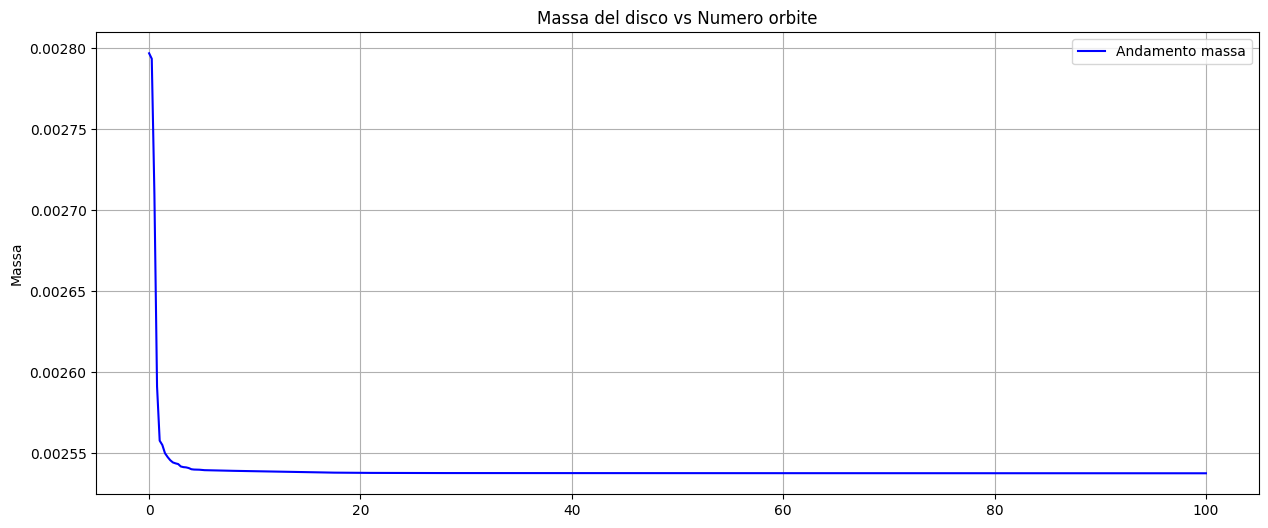
\includegraphics[width=\textwidth]{Immagini/Simulazioni/TestOpenouter.png}
    \caption{Andamento della massa del disco in funzione del numero di orbite. Notiamo che la perdita di massa avviene solamente durante le prime rivoluzioni del sistema binario: questo accade perché ad $r_{max}$ giungono delle spirali di materiale lanciate dal corpo perturbante mentre il disco caratterizzato dal profilo di densità $\sigma(r,\,0)$ viene distrutto.}
    \label{fig:test_openouter}
\end{figure}

Abbiamo effettuato un test per determinare quale fosse la combinazione di BC computazionalmente più efficace facendo evolvere lo stesso sistema per un numero fissato di orbite della binaria, variando solamente le condizioni al contorno su $v_r$.
\begin{table}[H]
\begin{center}
\begin{tabular}{|C{3cm}|C{3cm}|C{3cm}|}
\hline
\rowcolor{yellow}
 & OpenInner & Anti-simmetrico\\
\hline
\cellcolor{yellow} OpenOuter & 1h 34min 56s  & 1h 41min 13s\\
\hline
\cellcolor{yellow} Anti-simmetrico & 2h 3min 18s & 2h 13min 20s \\
\hline
\end{tabular}
\caption{Confronto fra le tempistiche d'esecuzione utilizzando diverse combinazioni di BC per la velocità radiale $v_r$. Le righe indicano le diverse scelte ad $r_{max}$, mentre le colonne quelle ad $r_{min}$.}
\label{tab:coor_Fargo3D}
\end{center}
\end{table}
Osserviamo che l'accoppiata \textit{open-open}, oltre ad essere fisicamente corretta, implica i tempi d'esecuzione minori. 

\subsection{Utilizzo del damping}

Nelle simulazioni effettuate con Fargo3D è possibile utilizzare una condizione al contorno che smorzi le perturbazioni di densità che si vengono a creare nelle regioni limitrofe alle frontiere della griglia (vedi sezione \ref{subsec:con_cont_far}). 

L'utilizzo del damping nelle simulazioni che vogliamo effettuare è rischioso poiché uno dei campi su cui esso agisce è la velocità azimutale del materiale costituente il disco. 
Modificare il valore di $v_{\theta}$ equivale ad applicare una coppia di forze: dato che il troncamento è determinato dall'equilibrio fra momenti torcenti, non vogliamo introdurne di artificiali.
Per verificare che il damping non dovesse essere utilizzato abbiamo effettuato due run, entrambe di lunghezza 20 orbite del sistema binario, simulando l'evoluzione del disco circum-secondario posto attorno ad una stella di massa pari ad $1/3$ di quella della primaria.
Notiamo (vedi Figura \ref{fig:si_no_dump}) come i risultati che otteniamo siano differenti nelle due casistiche.
L'immagine di sinistra presenta una corona circolare limitrofa alla frontiera esterna con densità maggiore rispetto a quella della regione svuotata attorno al disco.
Questo accade perché il damping oltre a porre delle condizioni sulle velocità del materiale, agisce anche sulla densità alterandone i valori.
Una conseguenza evidente dello smorzamento è la mancata formazione di un bordo netto del disco: mentre nella figura di destra la regione occupata dal gas risulta evidente, in quella di sinistra la parte esterna non è chiaramente delineata. Decidiamo quindi di lavorare senza damping.

\begin{figure}[h]
    \centering
    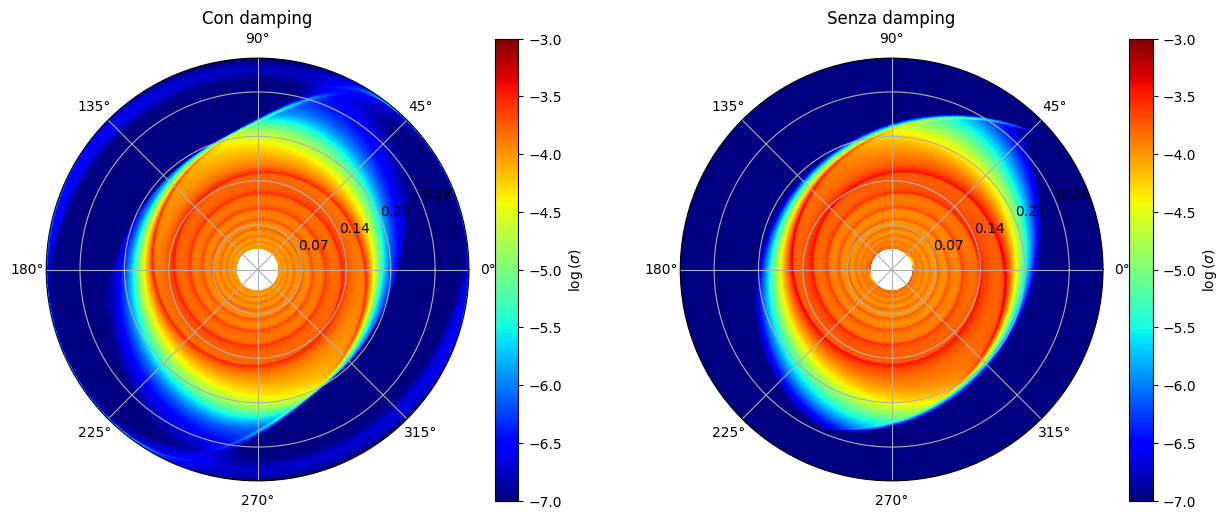
\includegraphics[width=\textwidth]{Immagini/Simulazioni/ConSenzaDamping.png}
    \caption{Confronto fra utilizzo e mancato utilizzo del damping. Notiamo che il disco quando viene applicato lo smorzamento non presenta una delimitazione precisa.}
    \label{fig:si_no_dump}
\end{figure}

\section{INDACO}

Le simulazioni necessarie per determinare le caratteristiche dei dischi circum-stellari richiedono l'utilizzo di un'elevata capacità computazionale: per questo motivo abbiamo utilizzato INDACO.

INDACO, acronimo di 'INfrastruttura di calcolo per il trattamento di DAti COmplessi', è un centro di calcolo messo a disposizione dall'Università di Milano come supporto alla ricerca scientifica.
Il supercomputer è organizzato in cluster di nodi che differiscono fra loro per potenza computazionale e per memoria disponibile. Nell'ambito di questa tesi abbiamo utilizzato i nodi 'light', ciascuno dei quali è costituito da due CPU da 16 cores 'Intel E5-2683V4   2.1 GHz' ciascuna.

INDACO utilizza 'slurm' come scheduler: il sistema di coda gestisce le richieste d'esecuzione ed assegna le risorse computazionali quando disponibili.

\subsection{Efficienza di parallelizzazione}

Supponiamo di eseguire un programma in parallelo su un numero $n$ di processori. Per quantificare quanto più rapida sia l'esecuzione parallela rispetto a quella sequenziale è possibile definire lo speedup $s_n$ come
\begin{equation}
s_n\,=\,\frac{T_1}{T_n},
\label{eq:speed_up}
\end{equation}
dove $T_1$ è il tempo d'esecuzione nel caso di utilizzo di un solo processore, mentre $T_n$ contempla la casistica con $n$ processori. Per valutare quanto sia efficiente la parallelizzazione, è possibile definire l'efficienza di parallelizzazione $e_{par}$
\begin{equation}
e_{par}\,=\,\frac{s_n}{n}
\label{eq:speed_up}
\end{equation}
Per determinare su quanti processori eseguire le simulazioni, abbiamo effettuato un test per valutare $e_{par}$ sui nodi \textit{Light} di INDACO.
Noi vogliamo valutare lo strong scaling, che consiste nel determinare quanto efficiente sia la parallelizzazione mantenendo fissata la dimensione del problema in analisi all'aumentare del numero di processori utilizzati.
La casistica opposta allo strong scaling è quella del weak scaling, che è ciò che si verifica se incrementando il numero di cores, la dimensione del problema affidata ad ogni singolo core rimane la stessa.

Per prima cosa abbiamo lanciato una run di controllo su un singolo core della durata di un'ora: mantenendo lo stesso problema, abbiamo poi aumentato il numero di cores utilizzati. In Figura \ref{fig:testeff_indaco} è riportato l'andamento osservato.
\begin{figure}[h]
    \centering
    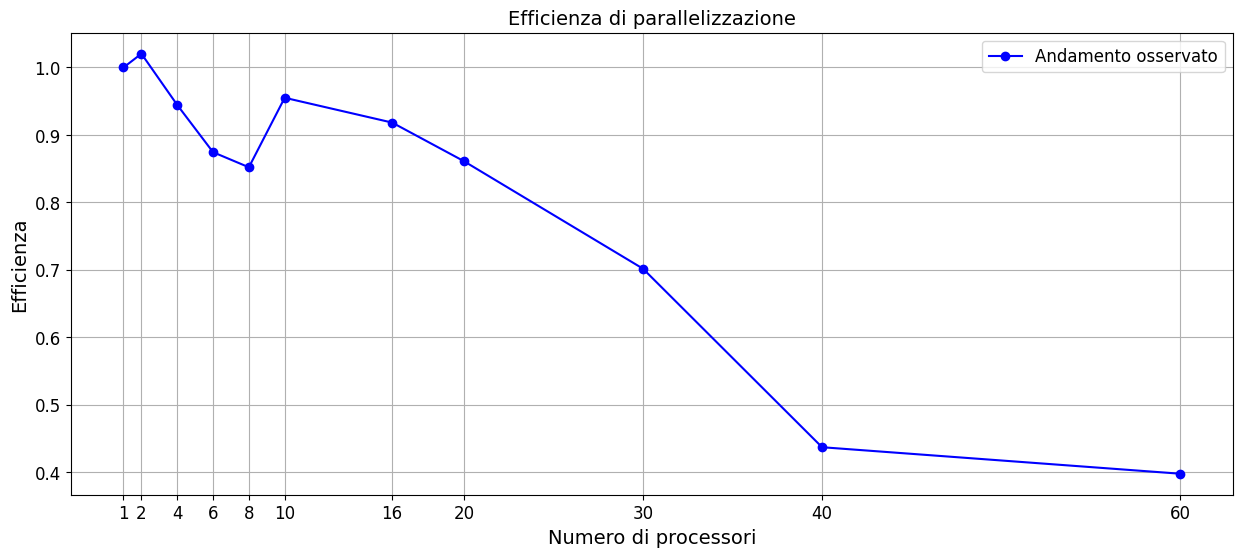
\includegraphics[width = \textwidth]{Immagini/Simulazioni/TestEfficienza_Indaco.png}
    \caption{Test di parallelizzazione effettuato su INDACO: stiamo testando lo strong scaling. Notiamo come dopo i 16 processori l'efficienza di parallelizzazione crolli drasticamente per assestarsi su valori del $40\%$: questo è dovuto alla maggiore complessità delle comunicazioni richieste, dettata dalla struttura dei nodi di INDACO.}
    \label{fig:testeff_indaco}
\end{figure}
Per come sono strutturati i nodi \textit{Light}, il programma viene eseguito sulla stessa CPU fino a quando il numero di cores selezionati è al massimo 16. Fra i 16 ed i 32 microprocessori utilizzati, i calcoli avvengono su un singolo nodo, ma coinvolgono entrambe le CPU delle quali è costituito. Infine se si impiegano più di 32 cores il programma viene eseguito su nodi differenti: le comunicazioni saranno più dispendiose e richiederanno maggior tempo.
Notiamo che per l'utilizzo di pochi cores la parallelizzazione non è molto efficiente: supponiamo che questo andamento sia dovuto al fatto che le sotto-griglie in cui viene suddiviso il dominio di simulazione presentino delle grandi regioni di contatto, il che rallenta l'esecuzione del codice.
\'E evidente un calo di prestazione fra i 16 ed i 32 cores: questo accade poiché è necessaria la comunicazione fra due parti differenti dello stesso nodo, che richiedono più tempo. 
Oltre i 32 cores l'efficienza di parallelizzazione si stabilizza sul $40\%$: i nodi coinvolti sono due, il che porta ad un aumento nella complessità delle comunicazioni. Il numero di microprocessori è ormai elevato ed è possibile che le sotto-griglie siano ormai troppo piccole per consentire un'esecuzione efficace del programma.
I motivi per cui abbiamo scelto di lavorare su 16 processori sono principalmente due:
\begin{list}{\textbf{-}}{\setlength{\itemsep}{0cm}}
    \item l'efficienza è superiore al $90\%$
    \item i programmi che possiamo eseguire simultaneamente su un singolo nodo di INDACO sono due. Questo ci consente di utilizzare tutta la potenza di calcolo ed al contempo di lavorare in modo efficiente
\end{list}

\section{Campionamento dello spazio dei parametri}

I parametri a cui siamo interessati per questo studio sono tre:
\begin{list}{\textbf{-}}{\setlength{\itemsep}{0cm}}
    \item la viscosità $\alpha$ del disco
    \item il rapporto fra le masse dei corpi costituenti la binaria $q\,=\,m_2/m_1$, dove $m_2$ è la massa della stella secondaria, mentre $m_1$ è quella della primaria.
    \item l'eccentricità della binaria $e$
\end{list}

Abbiamo deciso di valutare la dipendenza dalla viscosità del disco lavorando con:
\begin{equation}
\alpha\,=\,10^{-2},\,10^{-3},\,10^{-4}
\label{eq:par_space_vis}
\end{equation}
L'intervallo che ci siamo posti di esplorare è quello universalmente accettato come caratteristico dei dischi proto-planetari (vedi Sottosezione \ref{subsec: viscosity}).
Abbiamo lavorato con tre possibili scelte di $e$, rappresentanti le casistiche di binaria circolare, mediamente eccentrica e ad eccentricità elevata:
\begin{equation}
e\,=\,0.0,\,0.3,\,0.6
\label{eq:par_space_ecc}
\end{equation}
I valori di $q$ che abbiamo esplorato sono 4:
\begin{equation}
q\,=\,0.1,\,0.33,\,0.5,\,1
\label{eq:par_space_q}
\end{equation}
A viscosità fissata bisogna effettuare 21 simulazioni per studiare le caratteristiche dei dischi circum-stellari al variare di $q$ ed $e$. I tempi d'esecuzione $t_{es}$ dipendono fortemente dalla casistica considerata: abbiamo osservato che all'aumentare dell'eccentricità della binaria incrementa anche $t_{es}$. Fra le simulazioni caratterizzate da $e\,=\,0.0$ e quelle da $e\,=\,0.6$ i valori del tempo d'esecuzione aumentano di un fattore moltiplicativo $\sim 3$. Una simulazione su 16 processori viene effettuata in media in 16 ore.

\section{Metodi numerici per l'analisi dei risultati simulativi} \label{sec:metnum_anal}

In questa sezione presentiamo i metodi numerici che sono stati utilizzati per analizzare i dati prodotti dalle simulazioni. In primo luogo è necessario discutere le tecniche utilizzate per determinare massa, energia e momento angolare del disco.
Per evitare di introdurre errori numerici, è necessario ricordare le caratteristiche dei campi in FARGO3D: le grandezze scalari sono definite a centro cella, mentre quelle vettoriali ai bordi (vedi Sottosezione \ref{subsec:MeshField}).\\

\textbf{Calcolo della massa}\\

Per determinare la massa di gas contenuta nella griglia lavoriamo con $\sigma(r,\,t)$. In primo luogo dobbiamo valutare quale sia l'area delle singole celle $A_{cella}$: per effettuare questo calcolo sfruttiamo la simmetria della partizione utilizzata. Le celle sono poste su anelli concentrici: $A_{cella}$ può essere calcolata una volta nota l'area della corona circolare $A_{cor}$ alla quale appartiene.

I limiti delle varie corone circolari possono essere individuati generando linearmente (dato che stiamo utilizzando una divisione lineare in $r$, vedi Sezione \ref{sec:Setup_sim}) 385 valori fra $r_{min}$ ed $r_{max}$ compresi: così facendo le celle radiali saranno 384. Noti gli estremi è possibile valutare $A_{cor}$ come 
\begin{equation}
A_{cor}\,=\,\pi(r_{i+1}^2\,-\,r_{i}^2),
\label{eq:a_cor}
\end{equation}
dove $r_{i+1}$ ed $r_i$ sono gli estremi radiali della regione considerata.
Ricavate le aree delle corone, le singole celle che le costituiscono avranno $A_{cella}$ pari a $A_{cor}/1152$ poiché la partizione della coordinata angolare è anch'essa lineare.
Notiamo che $A_{cella}$ non è la stessa per ogni cella facente parte della griglia, ma ha una dipendenza sulla coordinata radiale.

Una volta note le varie aree è immediato il calcolo della massa di materiale, poiché basta sfruttare la definizione di densità
\begin{equation}
m_{cella}\,=\,\sigma_{cella} \cdot A_{cella}.
\label{eq:mass_cella}
\end{equation}
Il valore di $m_{cella}$ ha una dipendenza sul tipo di partizione radiale utilizzata: in Figura \ref{fig:mass_grid} riportiamo un esempio di calcolo del profilo di densità del disco, dove la dipendenza dall'area delle cellette utilizzate nella griglia non è presente.

\begin{figure}[h]
    \centering
    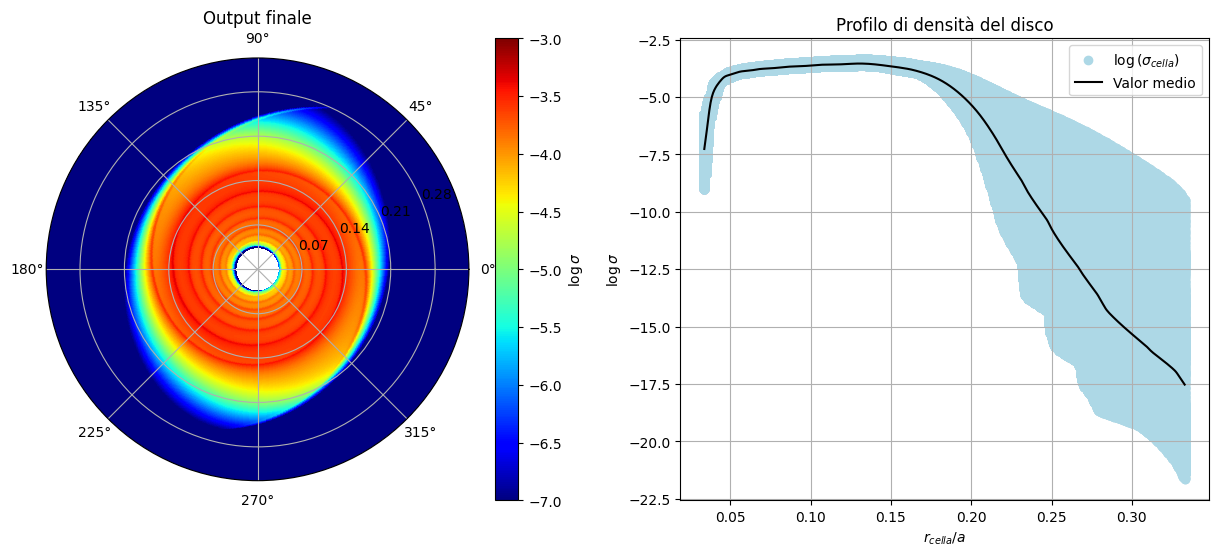
\includegraphics[width=\textwidth]{Immagini/Simulazioni/cal_mass.png}
    \caption{Calcolo del profilo di densità per il disco circum-secondario con $q\,=\,0.33$, $e\,=\,0.0$. L'output analizzato è quello alla cinquantesima orbita della binaria. La figura di sinistra mostra che valori assume il logaritmo di $\sigma$ nelle varie regioni della griglia. La Figura di destra riporta sovrapposti un grafico a disperisione di $\log{(\sigma_{cella})}$ ed il valor medio di tale quantità nelle varie corone circolari. Notiamo come nella regione più esterna della griglia l'intervallo in cui varia l'ordine di grandezza di $\sigma_{cella}$ è nettamente più ampio rispetto quanto accada per piccoli $r$. Per $r \simeq r_{min}$ il profilo di densità presenta un drop, dovuto alla presenza dello svuotamento artificiale.}
    \label{fig:mass_grid}
\end{figure}

\textbf{Energia meccanica}\\

L'energia meccanica per le celle viene calcolata come
\begin{equation}
E_{cella}\,=\,\frac{1}{2}m_{cella} \cdot(u_r^2\,+\,u_\theta^2)\,-\frac{m_{cella}}{r_{cella}}
\label{eq:ene_cella}
\end{equation}
dove $E_{cella}$ è l'energia della singola cella ed $r_{cella}$ è la coordinata radiale del centro della cella.
Nella \eqref{eq:ene_cella} $M_\ast$ e $G$ non compaiono poiché sono pari ad uno: il contributo potenziale dovuto al secondo corpo è trascurato poiché stiamo lavorando nella Roche-Lobe della stella al centro della griglia.
In Figura \ref{fig:ene_grid} è riportato un esempio di calcolo di $E_{cella}$: la quantità graficata è l'energia per unità di massa $E_{cella}/m_{cella}$.\\

\begin{figure}[h]
    \centering
    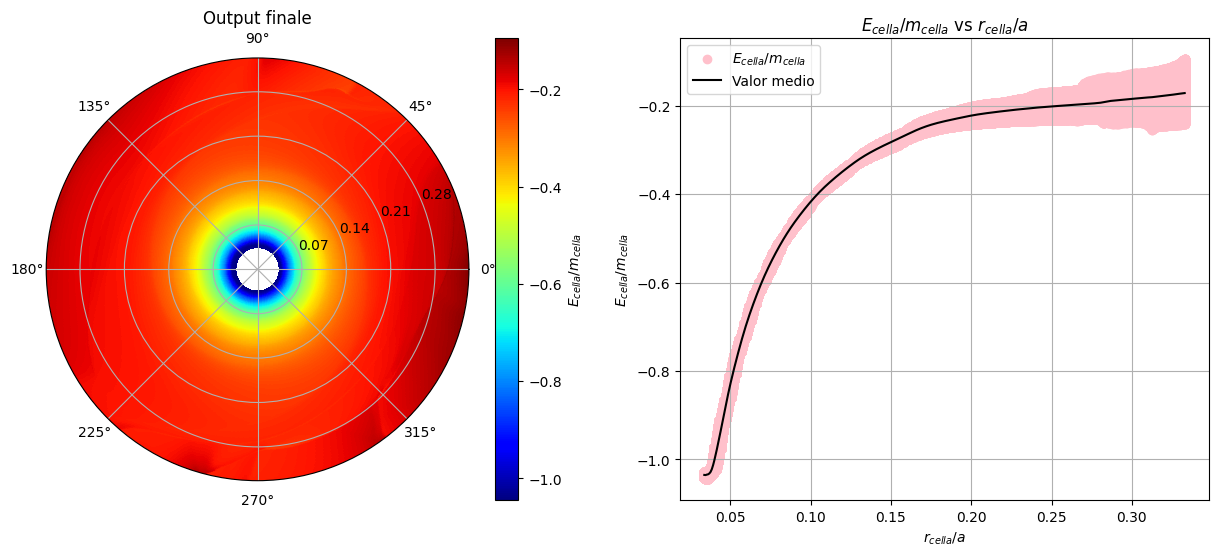
\includegraphics[width=\textwidth]{Immagini/Simulazioni/cal_ene.png}
    \caption{Calcolo dell'energia meccanica per unità di massa nel caso di disco circum-secondario con $q\,=\,0.33$, $e\,=\,0.0$. L'output analizzato è quello alla cinquantesima orbita della binaria. La figura di sinistra mostra che valori assume $E_{cella}/m_{cella}$ nella griglia. La Figura di destra riporta sovrapposti un grafico a dispersione di $E_{cella}/m_{cella}$ ed il valor medio nelle varie corone circolari. Notiamo che l'energia specifica è minore nella regione in cui è presente il materiale, poiché il gas è gravitazionalmente legato alla stella posta al centro della griglia.}
    \label{fig:ene_grid}
\end{figure}

\textbf{Momento angolare}\\

Il momento angolare della singola cella $L_{cella}$ viene calcolato tenendo conto della sola velocità azimutale come
\begin{equation}
L_{cella}\,=\,m_{cella} \cdot u_\theta \cdot r_{min-cella}
\label{eq:moma_cella}
\end{equation}
dove $r_{min-cella}$ è la coordinata radiale del bordo della cella a raggio minore. Lavorare con $r_{min-cella}$ è necessario poiché la velocità è un campo sfalsato in FARGO3D. In Figura \ref{fig:moma_grid} è riportato un esempio di calcolo di $L_{cella}$.

\begin{figure}[h]
    \centering
    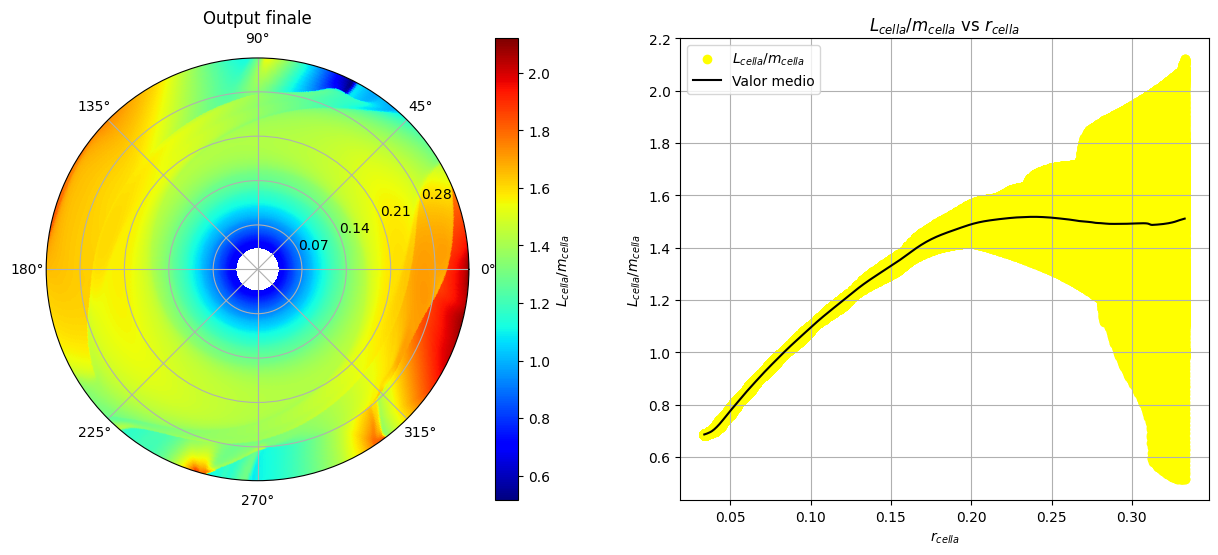
\includegraphics[width=\textwidth]{Immagini/Simulazioni/cal_moma.png}
    \caption{Calcolo del momento angolare per unità di massa nel caso di disco circum-secondario con $q\,=\,0.33$, $e\,=\,0.0$. L'output analizzato è quello alla cinquantesima orbita della binaria. La figura di sinistra mostra che valori assume $L_{cella}/m_{cella}$ nella griglia. La Figura di destra riporta sovrapposti un grafico a dispersione di $L_{cella}/m_{cella}$ ed il valor medio nelle varie corone circolari. Notiamo che a raggi $r_{cella} \geq 0.18\,a$ si hanno diversi valori di momento angolare per posizioni radiali fissate: possiamo pensare che lavorare in termini di semiassi maggiori d'orbita sia più corretto.}
    \label{fig:moma_grid}
\end{figure}

Vogliamo ora definire dei criteri che ci consentano di studiare le caratteristiche dei dischi: siamo in particolare interessati alle loro dimensioni ed alle loro eccentricità.

\subsection{Calcolo del raggio di troncamento}

Dobbiamo determinare un criterio che ci consenta di valutare le dimensioni della regione spaziale occupata dal disco: consideriamo come raggio di troncamento $r_T$ il semidiametro di quel cerchio centrato nell'origine del sistema di riferimento che contiene il $99.9 \%$ della massa di gas presente nel dominio simulato. Per calcolare tale raggio lavoriamo con le corone circolari concentriche che costituiscono la griglia. Valutiamo la massa progressiva come
\begin{equation}
M(R)\,=\,\sum_{r_{cella}<R} m_{cella},
\label{eq:m_prog}
\end{equation}
dove $R$ è un certo valore limite. Quando nella regione caratterizzata da $r_{cella}\,<\,R$ viene raggiunto il valore prefissato di massa abbiamo determinato il raggio di troncamento. In Figura \ref{fig:cal_dim} è riportato un esempio di calcolo di $r_T$.

\subsection{Calcolo del semiasse maggiore di troncamento}

Alcuni dischi circumstellari sono eccentrici: procedere con un metodo come quello esposto precedentemente implica commettere degli errori nella determinazione dell'effettiva dimensione del disco. Per ovviare a queste problematiche abbiamo calcolato il semiasse maggiore di troncamento $a_T$ come segue. In primo luogo si determina il valore del semiasse per ogni cella costituente la griglia. Dato che stiamo lavorando all'interno del Roche-Lobe, in prima approssimazione è possibile trascurare il contributo all'energia dovuto al corpo perturbante: per determinare $E_{cella}$ possiamo utilizzare i risultati ottenuti durante l'analisi del problema di Keplero (vedi Sezione \ref{sec:Keplero}). Il semiasse dell'orbita caratteristica del materiale contenuto nella singola cella è allora:
\begin{equation}
a_{cella}\,=\,-\frac{m_{cella}}{2\cdot E_{cella}}
\label{eq:sax_cella}
\end{equation}
Una volta calcolati tutti gli $a_{cella}$ si valuta la massa progressiva all'aumentare del semiasse limite $a_{lim}$: quando la regione interna ad $a_{lim}$ contiene il $99.9\%$ del materiale presente nel dominio simulato abbiamo determinato il semiasse maggiore di troncamento.
In Figura \ref{fig:cal_dim} è riportato un esempio di calcolo del semiasse di troncamento

\begin{figure}[h]
    \centering
    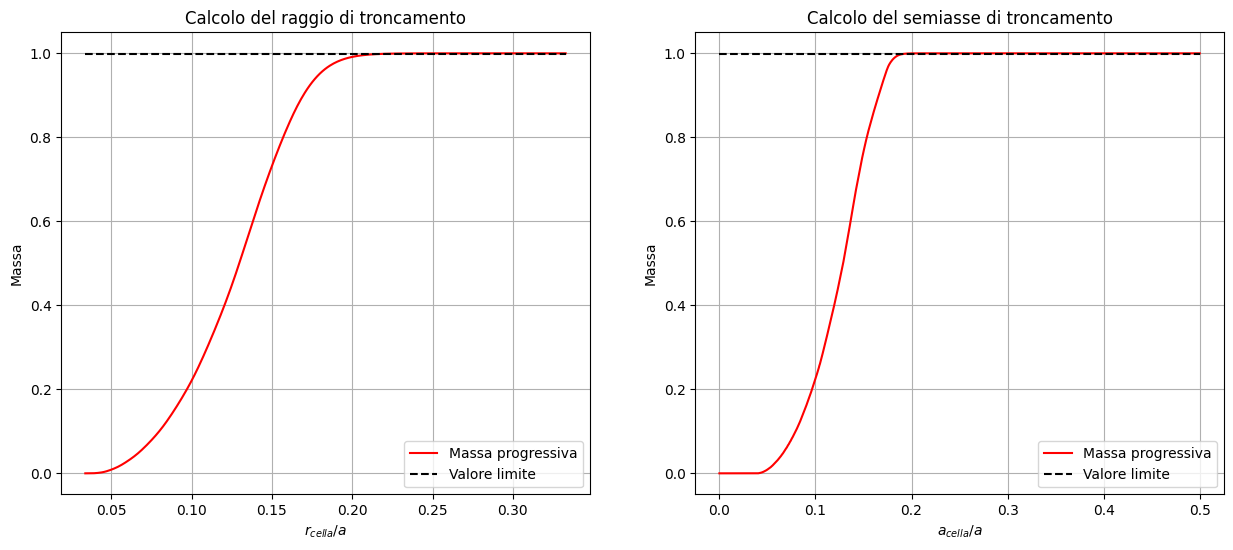
\includegraphics[width=\textwidth]{Immagini/Simulazioni/cal_dimdisco.png}
    \caption{Calcolo delle dimensioni del disco circum-secondario con $q\,=\,0.33$, $e\,=\,0.0$. L'output analizzato è quello alla cinquantesima orbita della binaria. La figura di sinistra riporta la massa cumulativa per la determinazione del raggio di troncamento. Per il disco analizzato abbiamo che $r_T\,=\,0.222\,a$. La figura di destra riporta la massa cumulativa per la determinazione del semiasse maggiore di troncamento. Per il disco analizzato abbiamo che $a_T\,=\,0.193\,a$.}
    \label{fig:cal_dim}
\end{figure}



\subsection{Calcolo dell'eccentricità del disco}

Un'informazione aggiuntiva sul disco può essere ricavata una volta note l'energia ed il momento angolare in tutta la griglia, come visto in Sezione \ref{sec:Keplero}. L'eccentricità dell'orbita viene calcolata come se la cella di materiale fosse una particella test ($m_{cella} \ll M_\ast$) 
\begin{equation}
e_{cella}\,=\,\sqrt{1\,-\,\frac{(r_{cella}\cdot u_\theta)^2}{a_{cella}}},
\label{eq:ecc_cella}
\end{equation}
dove abbiamo sfruttato il fatto che $M_\ast\,=\,1$.
Definiamo $e_{disco}$ come il valore medio di $e_{cella}$ nell'intorno di $a_T$, ossia consideriamo solamente quelle celle che hanno $a_{cella}$ confrontabile con il semiasse maggiore del disco. In Figura \ref{fig:cal_ecc} è riportato un esempio di calcolo dell'eccentricità del disco.

\begin{figure}[h]
    \centering
    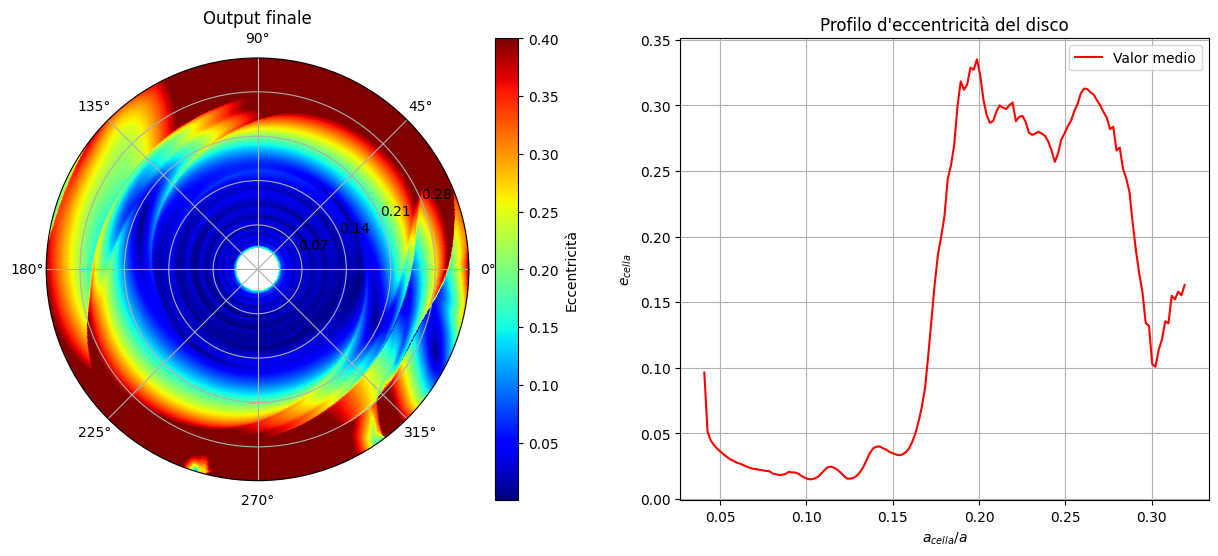
\includegraphics[width=\textwidth]{Immagini/Simulazioni/cal_ecc.png}
    \caption{Calcolo dell'eccentricità del disco circum-secondario con $q\,=\,0.33$, $e\,=\,0.0$. L'output analizzato è quello alla cinquantesima orbita della binaria. La figura di sinistra riporta i valori di eccentricità assunti dalle varie celle della griglia: abbiamo posto come limite massimo della scala di colore $e_{max}\,=\,0.4$. Notiamo che la regione ospitante la parte centrale del disco è caratterizzata da basse eccentricità, mentre il bordo dello stesso presenta valori di $e_{cella}$ maggiori. La Figura di destra riporta il profilo d'eccentricità del disco.}
    \label{fig:cal_ecc}
\end{figure}

\section{Simulazioni di convergenza}

Come esposto in Sezione \ref{sec:Setup_sim}, le simulazioni presenti in questo lavoro di tesi sono della lunghezza di 50 orbite della binaria.
La definizione che abbiamo deciso di adottare è di 384 celle radiali e 1152 angolari, entrambe con spacing lineare.
Le dimensioni della griglia che abbiamo utilizzato sono riportate in Tabella \ref{tab:dim_gr}.

Per determinare che le condizioni simulative con cui abbiamo lavorato non comportino la comparsa di errori sistematici, abbiamo effettuato tre tipi di run di convergenza per ogni valore del parametro $\alpha$ utilizzato.
Ci siamo concentrati su:
\begin{list}{\textbf{-}}{\setlength{\itemsep}{0cm}}
    \item lunghezza della simulazione
    \item dimensioni del raggio minimo della griglia
    \item definizione utilizzata
\end{list}

\subsection{Run Lunga}

Per verificare che cinquanta orbite del sistema binario fossero abbastanza per superare la fase di transitorio in cui si assiste alla distruzione della condizione iniziale, abbiamo effettuato tre simulazioni (una per ogni viscosità del materiale) dell'evoluzione del sistema per 500 periodi d'orbita delle due stelle.
Il disco d'accrescimento che abbiamo preso in considerazione è il circumsecondario caratterizzato da $m_2/m_1\,=\,0.33$ ed $e\,=\,0.0$: abbiamo osservato che la variazione delle dimensioni del disco è nell'ordine del $2/5\,\%$. I risultati ottenuti, riportati in Tabella \ref{tab:run_lunga}, sostengono la metodologia di lavoro che abbiamo implementato in questa tesi.

\begin{table}[H]
\centering
\begin{tabular}{|C{3cm}|C{2cm}|C{2cm}|C{2cm}|C{2cm}|}
\hline
\rowcolor{yellow}
Viscosità & \multicolumn{2}{|c|}{Raggi} & \multicolumn{2}{|c|}{Semiassi} \\
\hline
$\alpha$ & 50 orb. & 500 orb. & 50 orb. & 500 orb. \\
\hline
$\alpha\,=\,10^{-2}$ & $0.240\,a$ & $0.255\,a$ & $0.219\,a$ & $0.221\,a$ \\
\hline
$\alpha\,=\,10^{-3}$ & $0.222\,a$ & $0.217\,a$ & $0.194\,a$ & $0.192\,a$ \\
\hline
$\alpha\,=\,10^{-4}$ & $0.209\,a$ & $0.220\,a$ & $0.185\,a$ & $0.196\,a$ \\
\hline
\end{tabular}
\caption{Confronto fra le dimensioni dei dischi per 50 e 500 orbite.}
\label{tab:run_lunga}
\end{table}

In Figura \ref{fig:scal_rag} è riportato il valore del raggio di troncamento in funzione delle orbite effettuate dalla binaria per $\alpha\,=\,10^{-3}$: notiamo che la fase di equilibrio quasi-stabile viene raggiunta dopo le prime venti orbite.

\begin{figure}[h]
  \centering
  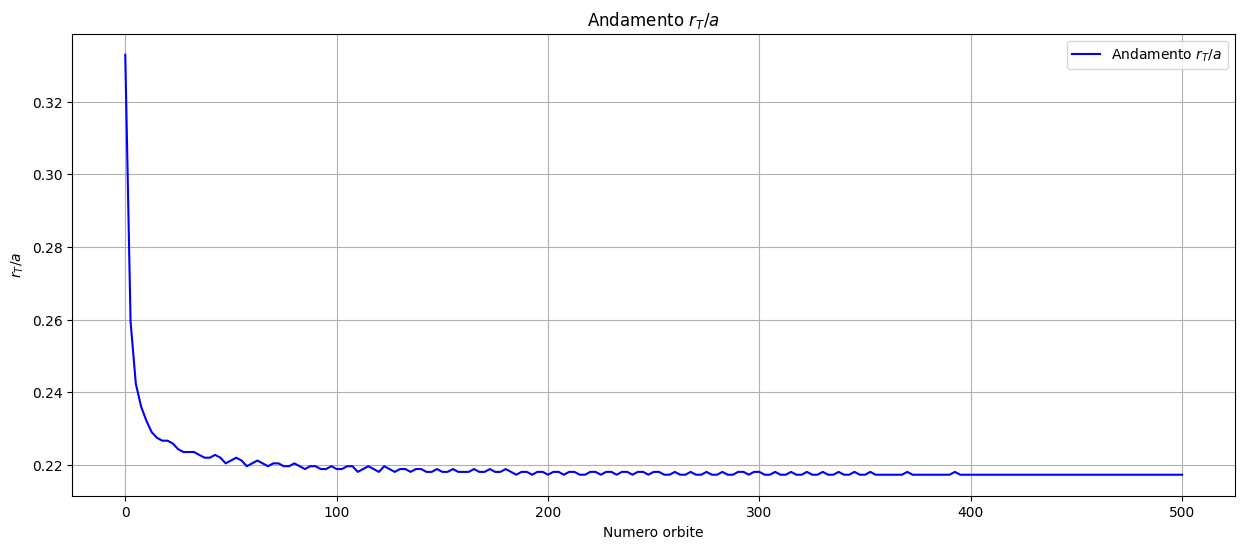
\includegraphics[width=\textwidth]{Immagini/Simulazioni/scal_rag.png}
  \caption{Esempio di dipendenza del raggio di troncamento dal numero di orbite della binaria: notiamo che il transitorio iniziale si esaurisce nelle prime venti orbite.}
  \label{fig:scal_rag}
\end{figure}

\subsection{Raggio minimo}

Notiamo che i dischi circum-secondari facenti parte dei sistemi binari ad elevata eccentricità sono di piccole dimensioni: vogliamo capire se lavorare con $r_{min}$ confrontabile con le dimensioni del disco stesso è un problema dal punto di vista numerico. Abbiamo effettuato tre simulazioni (una per ogni $\alpha$) del disco circum-secondario caratterizzato da $m_2/m_1\,=\,0.1$ ed $e\,=\,0.6$ utilizzando come valore di $r_{min}\,=\,0.033\,a$. Le dimensioni dei dischi nelle differenti casistiche analizzate sono riportate in Tabella \ref{tab:run_rmin}.

\begin{table}[H]
\centering
\begin{tabular}{|C{3cm}|C{2cm}|C{2cm}|C{2cm}|C{2cm}|}
\hline
\rowcolor{yellow}
Viscosità & \multicolumn{2}{|c|}{Raggi} & \multicolumn{2}{|c|}{Semiassi} \\
\hline
$\alpha$ & $r_{min}/2$ & $r_{min}$ & $r_{min}/2$ & $r_{min}$ \\
\hline
$\alpha\,=\,10^{-2}$ & $0.073\,a$ & $0.075\,a$ & $0.061\,a$ & $0.062\,a$ \\
\hline
$\alpha\,=\,10^{-3}$ & $0.069\,a$ &  $0.066\,a$ & $0.071\,a$ & $0.071\,a$ \\
\hline
$\alpha\,=\,10^{-4}$ & $0.060\,a$ & $0.064\,a$ & $0.056\,a$ & $0.058\,a$ \\
\hline
\end{tabular}
\caption{Confronto fra le dimensioni dei dischi per diversi raggi minimi della griglia simulativa.}
\label{tab:run_rmin}
\end{table}
In Figura \ref{fig:dim_rmin} sono riportati gli output finali per i differenti $r_{min}$ per $\alpha\,=\,10^{-4}$

\begin{figure}[h]
  \centering
  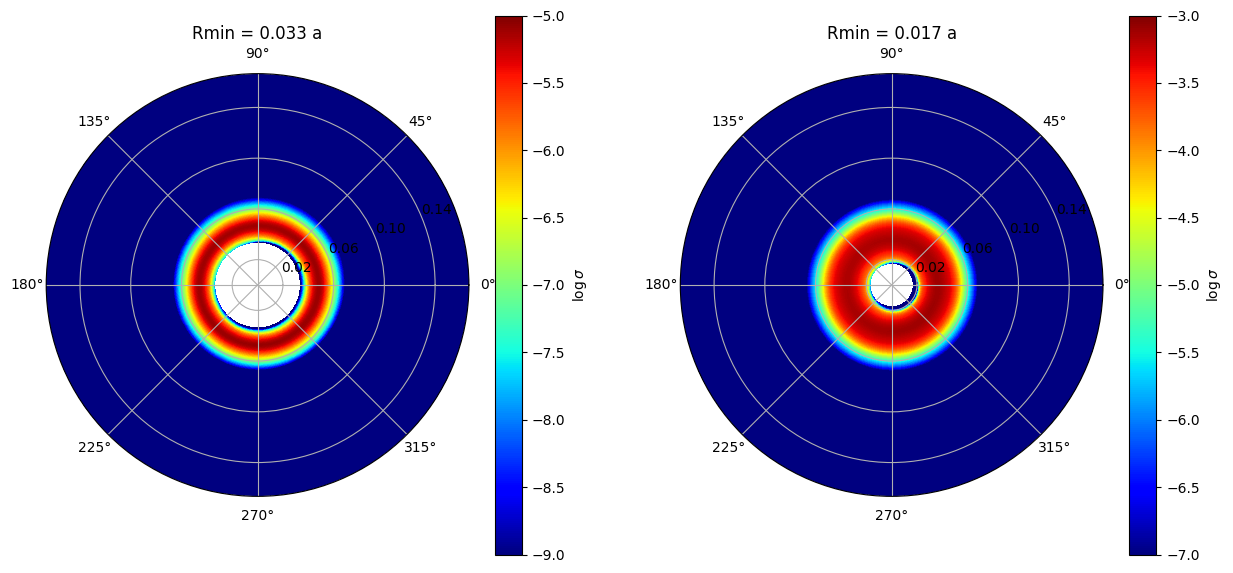
\includegraphics[width=\textwidth]{Immagini/Simulazioni/studio_rmin.png}
  \caption{Confronto fra il pattern di densità per $r_{min}\,=\,0.033\,a$ (figura di sinistra) ed $r_{min}/2\,=\,0.017\,a$ (figura di destra). Notiamo che, sebbene il disco simulato nella griglia con la frontiera interna posta ad $r_{min}$ risulti molto meno denso, la struttura dell'oggetto orbitante è la stessa ed i risultati ottenuti per le due simulazioni sono analoghi.}
  \label{fig:dim_rmin}
\end{figure}

\subsection{Alta risoluzione}

La terza caratteristica a cui siamo interessati con le run di convergenza è lo studio della definizione alla quale abbiamo lavorato. Per questo motivo effettuiamo tre simulazioni (una per ogni $\alpha$) ad una risoluzione più elevata, lavorando con $n_r\,=\,768$ ed $n_\varphi\,=\,2304$: abbiamo raddoppiato il numero di cellette sia per la coordinata radiale che per quella angolare. 
Il disco su cui ci concentriamo è il circum-secondario caratterizzato da $m_2/m_1\,=\,0.33$ ed $e\,=\,0.0$.
Le dimensioni ottenute sono riportate in Tabella \ref{tab:run_highdef}: dato che i risultati sono confrontabili, decidiamo di lavorare con $n_r\,=\,384$ e $n_\varphi\,=\,1152$ poiché è la scelta computazionalmente più efficace.

\begin{table}[H]
\centering
\begin{tabular}{|C{3cm}|C{2cm}|C{2cm}|C{2cm}|C{2cm}|}
\hline
\rowcolor{yellow}
Viscosità & \multicolumn{2}{|c|}{Raggi} & \multicolumn{2}{|c|}{Semiassi} \\
\hline
$\alpha$ & Normale & Alta & Normale & Alta \\
\hline
$\alpha\,=\,10^{-2}$ & $0.240\,a$ & $0.243\,a$ & $0.218\,a$ & $0.222\,a$ \\
\hline
$\alpha\,=\,10^{-3}$ & $0.222\,a$ & $0.229\,a$ & $0.194\,a$ & $0.200\,a$ \\
\hline
$\alpha\,=\,10^{-4}$ & $0.212\,a$ & $0.220\,a$ & $0.185\,a$ & $0.193\,a$ \\
\hline
\end{tabular}
\caption{Confronto fra le dimensioni dei dischi per diverse definizioni.}
\label{tab:run_highdef}
\end{table}

In Figura \ref{fig:dim_highres} riportiamo un esempio di configurazione finale nel caso della run ad alta risoluzione effettuata con $\alpha\,=\,10^{-2}.$

\begin{figure}[h]
  \centering
  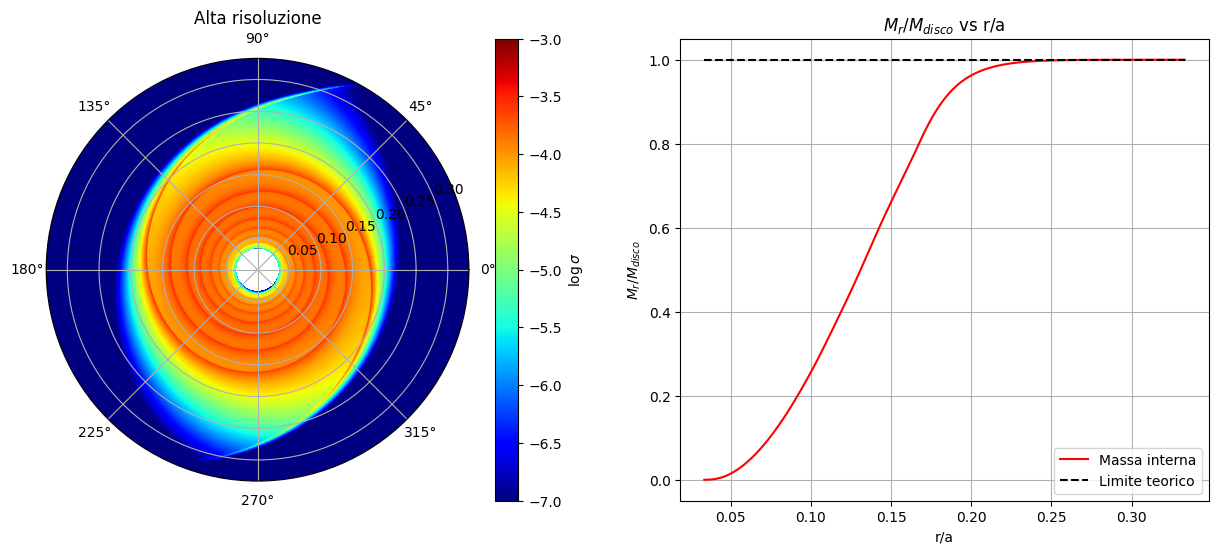
\includegraphics[width=\textwidth]{Immagini/Simulazioni/altadef.png}
  \caption{Configurazione finale per la run ad alta definizione con $\alpha\,=\,10^{-2}$.}
  \label{fig:dim_highres}
\end{figure}
